\documentclass{article}
\usepackage[utf8]{inputenc}
\usepackage{multicol}
\usepackage{mathpazo}
\usepackage{textcomp}
\usepackage{amsmath}
\usepackage{mdframed}
\usepackage{xcolor}
\usepackage{hyperref}
\usepackage{graphicx}
\usepackage[landscape=true]{geometry}

\definecolor{astral}{RGB}{176, 224, 230}
\definecolor{lred}{HTML}{EFAAAA}

\title{Computational Biology}
\author{Gian Hiltbrunner}
\date{January 2020}

\begin{document}

\begin{multicols*}{3}

\maketitle

\begin{mdframed}[backgroundcolor=lred] 
    \textbf{Disclaimer}\\
    Parts of the information provided within this document may be incomplete and/or incorrect.\\For corrections please submit a pull request at:
    \url{http://github.com/protelescristata/SummaryComputationalBiology}
\end{mdframed}

\section{Substitution Rate Matrices}

\subsection{JC69}
\begin{itemize}
    \item  All substitutions have the same rate $\lambda$
    \item 1 parameter
\end{itemize}

\begin{center}
    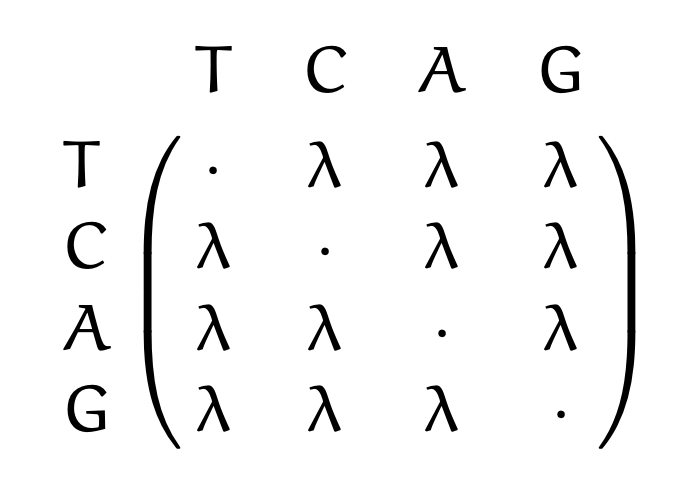
\includegraphics[width=0.5\linewidth]{js69.png}
\end{center}

\subsection{K80}
\begin{itemize}
    \item This model differentiates between transitions (T-C/A-G) and transversions. 
    \item 2 parameters
\end{itemize}

\begin{center}
    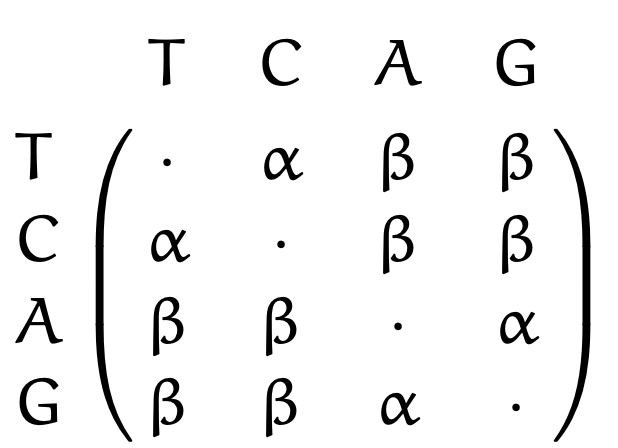
\includegraphics[width=0.5\linewidth]{k80.png}
\end{center}

\subsection{TN93}
\begin{itemize}
    \item Transitions between T/C happen with rate $\alpha_1 \times \pi$
    \item Transitions between A/G happen with rate $\alpha_2 \times \pi$
    \item Transversions happen with rate $\beta\times \pi$
    \item 3 + 3 ($\pi_x$) parameters 
\end{itemize}

\begin{center}
    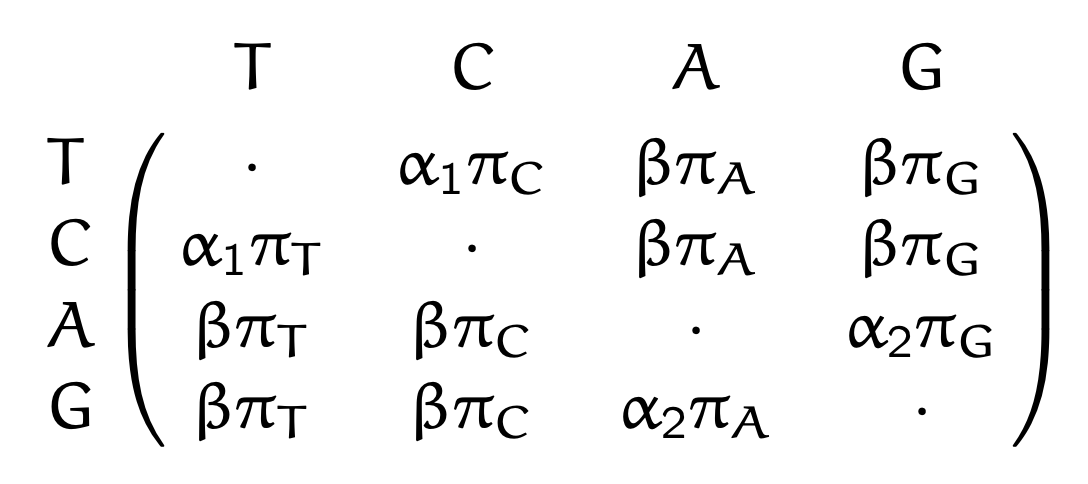
\includegraphics[width=0.7\linewidth]{tn93.png}
\end{center}

\begin{itemize}
    \item If $\alpha_1 = \alpha_2$, the model is named \textbf{HKY}
\end{itemize}

\subsection{GTR - Generalised Time Reversible}

\begin{itemize}
    \item[+] quite flexible
    \item[+] time-reversible
    \item[-] not completely general
    \item 6 + 3 ($\pi_x$) parameters 
\end{itemize}

\begin{center}
    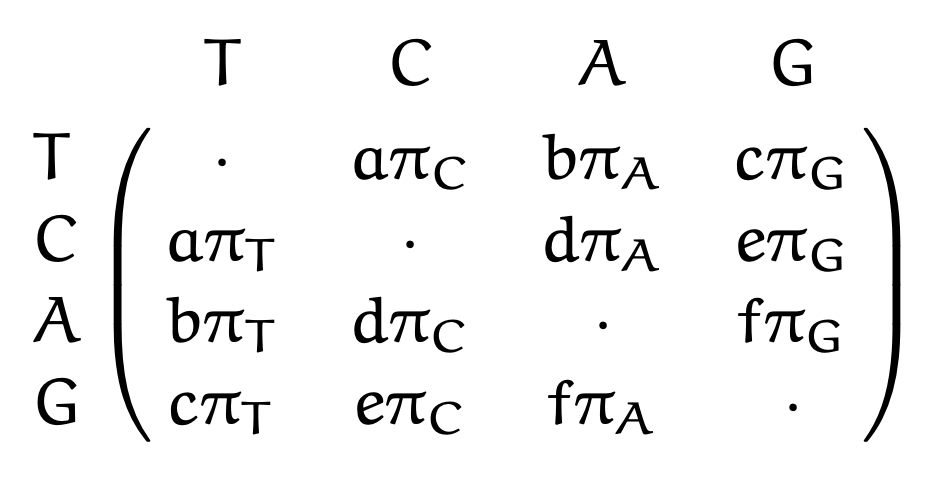
\includegraphics[width=0.7\linewidth]{GTR.png}
\end{center}
\subsection{UNREST}

\begin{itemize}
    \item Unrestricted model 
    \item Each substitution has a different rate
    \item[+] Most general model 
    \item[+] Other models are special cases of UNREST
    \item[-] Mathematically complicated to handle
    \item[-] Not time-reversible
    \item 12 parameters 
\end{itemize}

\begin{center}
    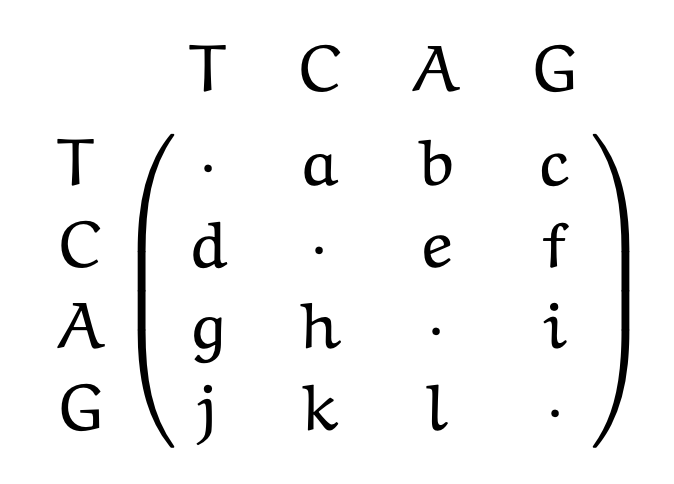
\includegraphics[width=0.5\linewidth]{unrest.png}
\end{center}

\section{Calculating Sequence Distance}
\subsection{Transition Probability Matrix}
\label{transprobmat}

Using the substitution rate matrix $Q$ we derive the transition probability matrix $P(t)$, which gives the probabilities of nucleotide $i$ changing to nucleotide $j$ in any time interval $t$.

\begin{center}
    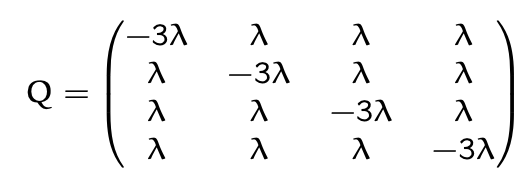
\includegraphics[width=0.5\linewidth]{substitutionratematrix.png}
\end{center}

$$P(t) = \text{e}^{Qt}$$

\begin{center}
    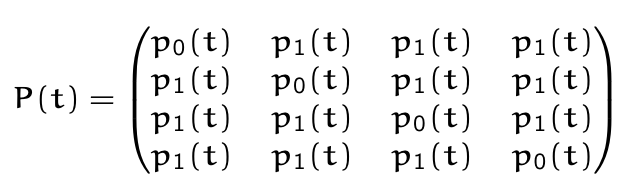
\includegraphics[width=0.7\linewidth]{transitionprobabilitymatrix.png}
\end{center}

\subsection{Stationary Distribution}

\begin{itemize}
    \item For $t \rightarrow \infty$ we reach a stationary distribution; where the transition probabilities all tend towards $0.25$. 
    \item Any long sequence will thus be composed of equal amounts of T,C,A and G at $t \rightarrow \infty$
\end{itemize}

\section{Maximum Likelihood Estimators}
\begin{mdframed}[backgroundcolor=astral] 
    \textbf{Likelihood Function}\\
    Describes a hypersurface whose peak represents the combination of model parameter values that maximize the probability of drawing the obtained sample. 
\end{mdframed}

\begin{mdframed}[backgroundcolor=astral] 
    \textbf{Maximum Likelihood Estimator}\\
    Is an estimator of a model parameter that maximises the probability to obtain the observed results.
\end{mdframed}

\textbf{Example}: Estimate the probability that a die shows side 6. \textrightarrow The die is thrown $n = 100$ times and we obtained a 6 $x = 40$ times. 
\begin{itemize}
    \item Define probability of throwing a 6 $x$ times out of $n$ tries \textrightarrow Binomial-distribution, thus: $P = {n\choose x}p^x(1-p)^{n-x}$, where $p$ is the probability of throwing a 6
    \item We use this probability as our likelihood function and plug in the given values: $L(p;x) = {100\choose 40}p^4^0(1-p)^6^0$
    \item To find the maximum likelihood we calculate the first derivative of our likelihood function and set $L' = 0$ to find the maximum. 
    \item Transformations are sometimes applied to the likelihood function. e.g.: $l(p;x) = \log (L(p;x))$
    \item We estimate the probability by solving for $p$ and get $p = 0.4 \neq 1/6$
\end{itemize}

\subsection{Confidence Intervals}

Interval which tries to capture the uncertainty of a parameter estimate. 

\begin{mdframed}[backgroundcolor=astral] 
    \textbf{Confidence Interval}\\
    If a parameter is repeatedly estimated from realisations of the random experiment and the interval estimate for each realisation, we expect 95 \% of these intervals to contain the true parameter.
\end{mdframed}

Confidence intervals may be calculated on the basis of likelihood intervals.\\
Let $X$ be a random variable with a distribution parametrised in $\theta$. Based on collected data $x$ of a huge sample, the maximum likelihood estimation for the parameter is $\hat{\theta}$. Then, $2(l(\hat{\theta} - l(\theta)) \sim x^2_k$
\begin{itemize}
    \item Determine the value of the log likelihood function in $\hat{\theta}$: $l(\hat{\theta};x)$
    \item Calculate $l(\hat{\theta};x) - 0.5x^2_{k,5\%}$; subtract half of the $5\%$ most extreme values according to the $x^2$-distribution
    \item Determine those $\theta$ values for which the the following holds: 
    $l(\theta;x) = l(\hat{\theta};x) - 0.5x^2_{k,5\%}$
\end{itemize}

\subsection{MLE for Sequence Distance}
The MLE framework can be used to derive a maximum likelihood estimation for the sequence distance under a JC69 model. 
We have the transition probability matrix as seen in subsection (\ref{transprobmat}) with:
\begin{align*}
    p_0(t) = \frac{1}{4} + \frac{3}{4}\text{e}^{-4\lambda t}\\
    p_1(t) = \frac{1}{4} + \frac{1}{4}\text{e}^{-4\lambda t}
\end{align*}
For two sequences of length $n$ with $x$ differences the probability that any one position is different is $p = 3p_1(t)$. We define $d = 3\lambda t$ as the expected distance in time $t$ and get for the probability that $x$ out of $n$ positions are different: \begin{align*}
L(d;x) = {n \choose x} p^{x}(1-p)^{n-x}=\\
{n \choose x}
\left(\frac{3}{4}-\frac{3}{4} e^{-\frac{4}{3} d}\right)^{x}\left(\frac{1}{4}+\frac{3}{4} e^{-\frac{4}{3} d}\right)^{n-x}
\end{align*}
\begin{itemize}
    \item We compute $l(d;x) = \log(L(d;x))$
    \item An calculate the first derivative $\hat{d} = l'(d;x)$⁄⁄
\end{itemize}

Which gives us the MLE of the JC69 distance: 
$$\hat{d} = -\frac{3}{4}\log\left(1-\frac{4x}{3n}\right)$$

\subsection{Example of JC69 MLE}

\begin{center}
    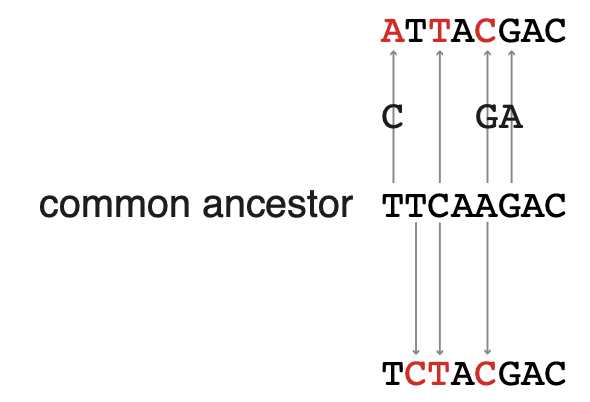
\includegraphics[width=0.5\linewidth]{mlejc69.png}
\end{center}

\begin{itemize}
    \item Length of gene: $n = 8$
    \item Differences between the two sequences: $x = 2$
\end{itemize}

$$\hat{d} = -\frac{3}{4}\log\left(1-\frac{4\times 2}{3\times 8}\right) = 0.3$$
Determine the $95 \%$ confidence interval for the given parameters. 

\section{Variable Substitution Rates}

\begin{itemize}
    \item Not all sites evolve at the same rate
    \item Mutation rates may vary across sites \item The acting selection in the phenotypic level exerts different evolutionary pressure on different sites
\end{itemize}
\end{multicols*}
\end{document}
